\subsection{Interfaces existantes} \label{sec:interfaces_existantes}

\subsubsection{Monitor3.0}
\textbf{Monitor3.0} est une interface développée en C++ permettant de se connecter à l'e-puck2 via Bluetooth \autocite{noauthor_e-puck2monitor_2024} ou par Wi-Fi.
Elle offre plusieurs fonctionnalités-clés :
\begin{enumerate}
    \item accès au flux vidéo de la caméra avec possibilité de modifier les paramètres d'enregistrement,  
    \item contrôle des \acrshort{led}s,  
    \item diffusion de sons pré-enregistrés via le haut-parleur intégré,  
    \item déplacement du robot dans diverses directions,  
    \item captation des sons ambiants par les trois microphones,  
    \item analyse des données fournies par l'\acrshort{imu} et
    \item consultation des relevés des capteurs infrarouges et du capteur de lumière ambiante.  
\end{enumerate}

\begin{figure}[H]
    \centering
    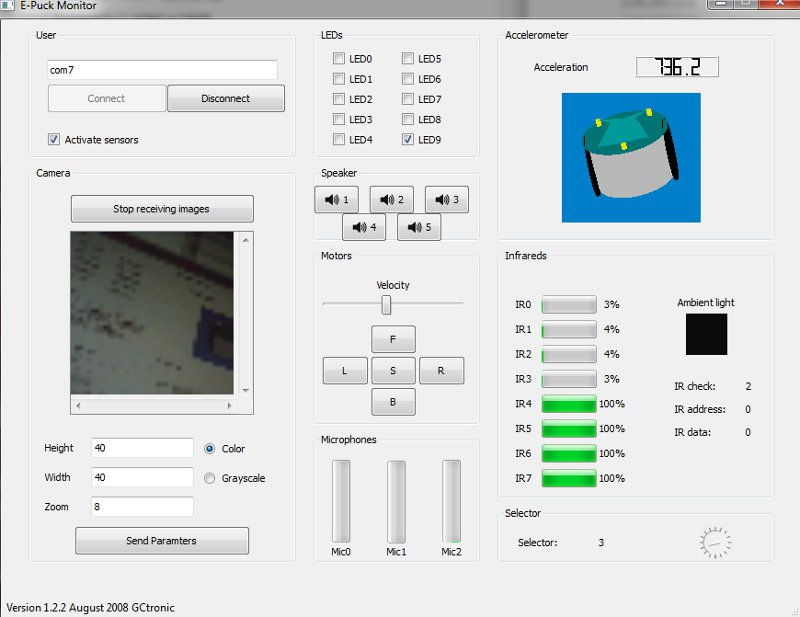
\includegraphics[width=0.6\linewidth]{figures//Monitor3.0.png}
    \caption{Capture d'écran de l'interface PC \autocite{gctronic_e-puck2_nodate}}
    \label{fig:screenshot_monitor_interface}
\end{figure}

Ce logiciel semble répondre aux besoins premiers de prendre le contrôle du robot et de ses fonctionnalités principales. 
Cependant, il présente certaines restrictions:
\begin{itemize}
    \item pas de prise en charge des extensions matérielles ajoutées à l'e-puck2 ;
    \item liste de fonctionnalités relativement restreintes par rapport aux besoins (e.g. communication inter-robots, déplacements aléatoires ou pré-programmés, retours visuels sur l'état, ...) ;
    \item interface obsolète, inadaptée aux évolutions actuelles de la recherche et de l’enseignement, et peinant à motiver ou susciter la curiosité nécessaires pour engager activement les utilisateurs avec le robot.
\end{itemize}

\subsubsection{Prototype de cartographie}
Dans une vidéo démontrant une phase de test pour le Pi-puck, on observe que GCTronic a développé un prototype d'application mobile pour Android permettant de suivre en temps réel les déplacements d'un robot dans une arène \autocite{gctronic_pi-puck_nodate}.

Malgré plusieurs recherches sur le sujet, il n'existe actuellement aucune application mobile officielle, suffisamment connue ou open-source, permettant de contrôler un ou plusieurs robots e-puck2.
Cela révèle ainsi un besoin caché du domaine, d'autant plus que les jeunes générations montrent une aisance particulière avec les outils numériques puisque ceux-ci ont pris une place à multiples facettes dans leur approche de la vie et de leurs relations sociales \autocite{tully_growing_2003}.

\subsubsection{Conclusion}
Bien que Monitor3.0 offre un premier niveau d'interaction avec l'e-puck2, son manque de flexibilité et son incompatibilité avec les extensions récentes soulignent la nécessité d'une solution plus évolutive et adaptée aux besoins actuels.

De plus, l'absence d'applications mobiles dédiées représente une opportunité à explorer dans le futur, une piste intéressante pour le développement d'outils plus accessibles et adaptés aux usages actuels.
